\documentclass{article}
\usepackage[utf8]{inputenc}
\usepackage[ngerman]{babel}
\usepackage{cite}
\usepackage{graphicx}
\usepackage{hyperref}
\usepackage{csquotes}
\usepackage{float}
\usepackage{placeins}
\usepackage[official]{eurosym}

\title{\enquote{WolkeSieben} - die Cloud-Native Tiervermittlung}
\author{Klaus Fuhrmeister, Arne Müller, Niklas Sauer, Savina Diez}
\date{Februar 2021}


\begin{document}

\maketitle

\section{Motivation und Idee} % Savina

Tiere aller Art verdienen ein fürsorgliches und sicheres Umfeld. Leider kann dies nicht stets garantiert werden, in anderen Fällen funktioniert das nur für eine bestimmte Anzahl von Artgenossen. Daher leisten Tiervermittlungen wie \href{https://www.ebay-kleinanzeigen.de/s-haustiere/c130}{Ebay Kleinanzeigen} oder \href{https://www.tiervermittlung.de}{Tiervermittlung.de}  einen wichtigen Beitrag für unsere Gesellschaft. Auch wir, ein Team von Tierliebhabern, möchten uns dem anschließen, dies jedoch mit einer ansprechenden Benutzeroberfläche, intuitiven Funktionen und einer Infrastruktur tun, die theoretisch alle Vermittlungen der Welt übernehmen kann. Angesichts dieser Vorlesung, soll letzteres mit Hilfe der Google Cloud Plattform erreicht werden.

Das Portal mit dem Decknamen \enquote{WolkeSieben} erlaubt aktuellen Besitzern Angebote zu erstellen, diese mit Bildern und Videos zu versehen, hierzu Anfragen zu erhalten und Details mit Interessenten in Echtzeit zu besprechen. Durch das Hosting in der Cloud können daneben noch einige weitere Features effizient und skalierbar umgesetzt werden. Allgemein erlaubt diese Form des Hostings natürlich einen Geräte-, zeit- und ortsunabhängigen Zugriff, sowie bessere Kostenstrukturen, da die Hardware, sowie die Wartung der Ressourcen entfallen.

Im Rahmen dieser Arbeit erläutern wir wie eine Vielzahl von Google Cloud Services zum Funktionsumfang und der Bereitstellung unserer Plattform beitragen werden. Zur besseren Übersicht, folge eine kurze Zusammenfassung:

\begin{itemize}
    \item \textbf{Cloud Run} zur Bereitstellung zweier Microservices
    \item \textbf{App Engine} zur Bereitstellung eines dritten Microservice
    \item \textbf{Cloud CDN} zur Bereitstellung des Frontends
    \item \textbf{Cloud Firestore} zur Speicherung von Chat-Daten
    \item \textbf{Cloud Memorystore} zur Skalierung des Echtzeit-Chats
    \item \textbf{Cloud BigTable} zur Speicherung von \enquote{Gefällt mir} Angaben
    \item \textbf{Cloud SQL} zur Speicherung von Benutzer Profilen, Angeboten, Merklisten, sowie Rassen-Abonnements
    \item \textbf{Cloud Storage} zur Speicherung von statischen Dateien wie dem Frontend, Profil- / Angebots-Medien und einer Admin-Oberfläche
    \item \textbf{Cloud Functions} zur Benachrichtigung über neue Angebote von abonnierten Rassen
    \item \textbf{Cloud Pub/Sub} zum Auslösen der o.g. Benachrichtigungen
\end{itemize}

\begin{figure}[htbp]
\centering
\label{fig:homepage}
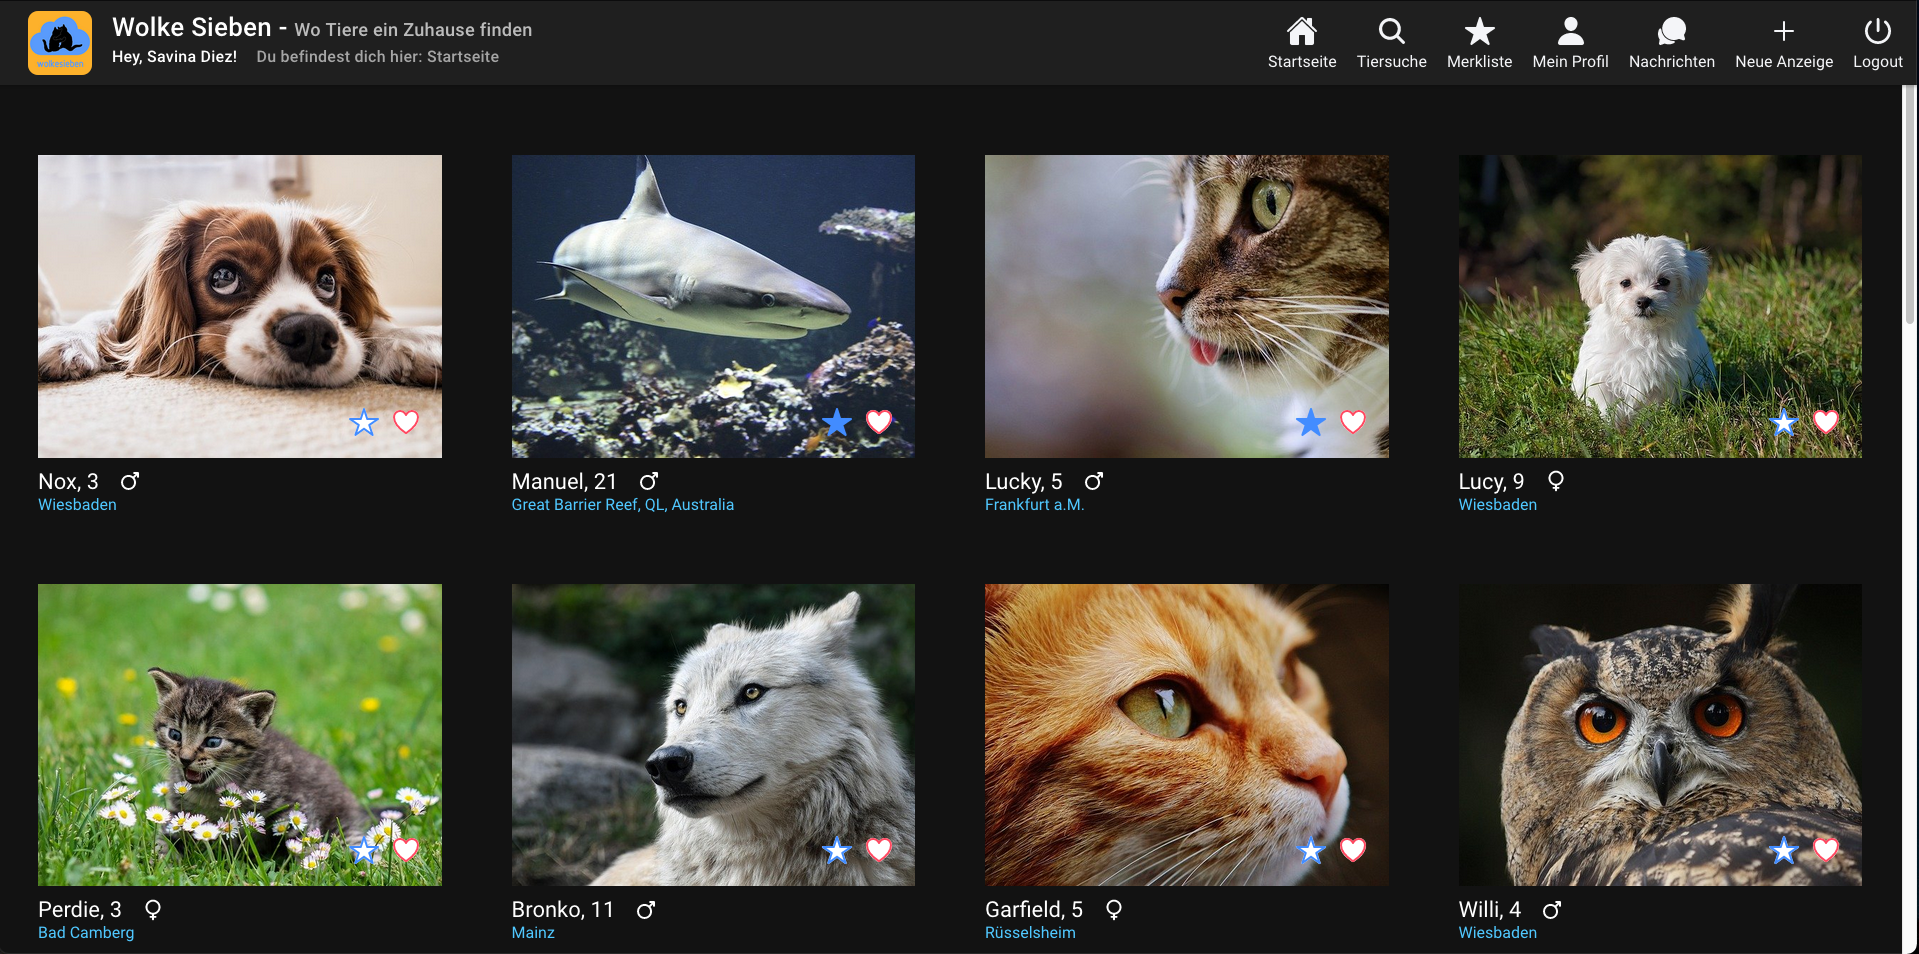
\includegraphics[width=\textwidth]{images/homepage}
\caption{Startseite von \href{https://cc-wolkesieben.de}{cc-wolkesieben.de}}
\end{figure}

Der Prototyp unserer Applikation, wie in Abbildung \ref{fig:homepage} demonstriert, ist ab sofort unter folgender Adresse aufrufbar: \url{https://cc-wolkesieben.de}.

% Why leverage cloud computing? Comparison to alternative hosting methods

\section{Architektur} % Arne
\subsection{Microservices}

Wie für Cloud-Anwendungen üblich, setzen wir bei der Struktur des Backends auf einen Microservice-Ansatz bei dem die ganzheitliche API in verschiedene, voneinander unabhängige Programme aufgeteilt wird. Diese Form der Bereitstellung hat einige Vorteile, die hier nochmal herausgestellt werden sollen.

Zum einen können die einzelnen Funktionen auf diese Weise in Umgebungen bereitgestellt werden, welche speziell auf diese zugeschnitten sind. In unserer Anwendung sieht man dies primär anhand der Aufteilung nach den verwendeten Datenbank-Typen (Polyglott Persistency). Im Umkehrschluss muss sich jeder Microservice somit auch nur mit denen für seine Domäne relevanten Technologien befassen. Die erleichtert die Konfiguration und trägt dazu bei, dass sich Services einfacher unter den Entwicklern eines Team aufteilen lassen, ohne dass diese sich in die Quere kommen. Zu guter Letzt lassen sich die Möglichkeiten der Bereitstellung in der Cloud so optimal ausnutzen, da jeder Microservice auf der Infrastruktur aufgesetzt werden kann, die für ihn am geeignetsten ist, ohne den Rest der Anwendung auf einen Kompromiss zu forcieren. Dies wiederum erlaubt die unabhängige Skalierung der am meisten nachgefragten Teilbereiche, d.h. Microservices, der ganzheitlichen API.

\begin{figure}[H]
\centering
\label{fig:architecture}
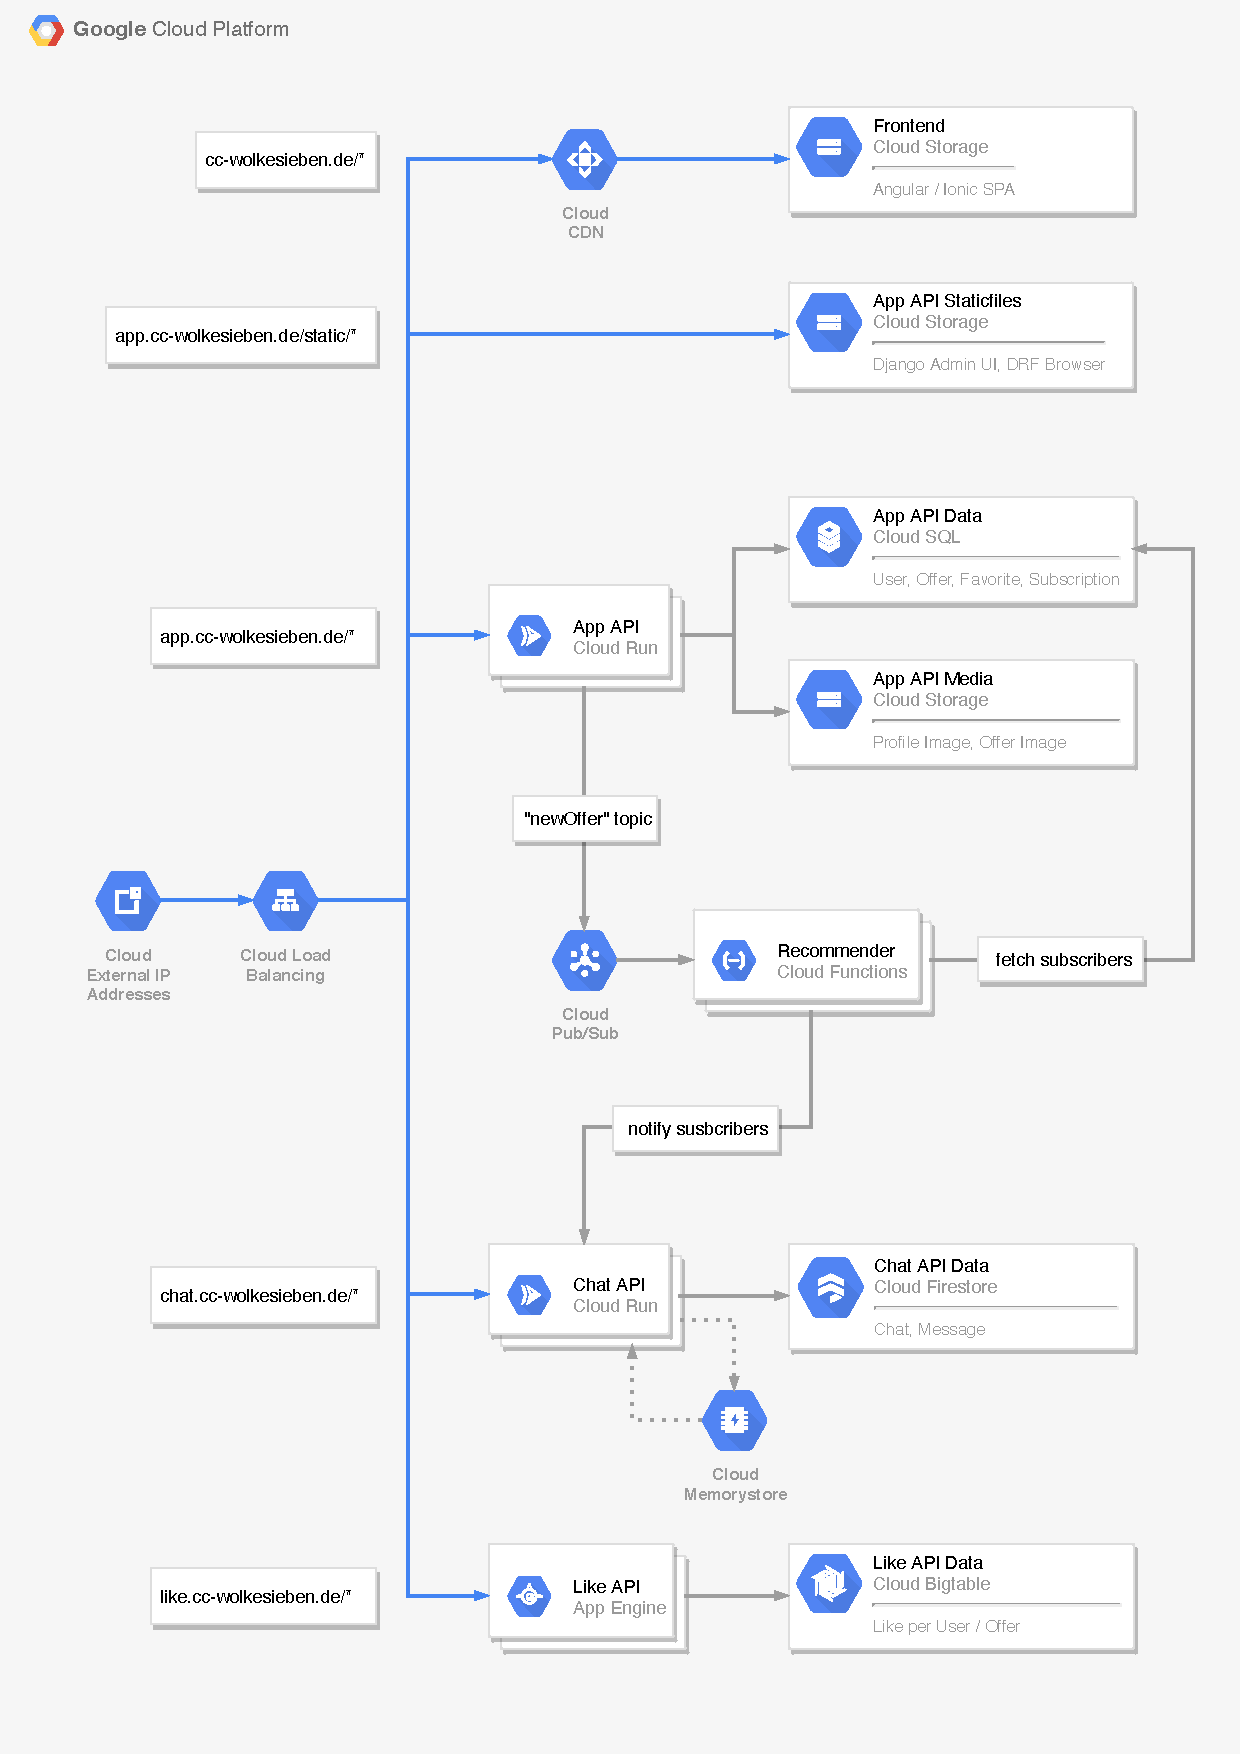
\includegraphics[width=\textwidth]{images/gcp-architecture}
\caption{Architekturüberblick}
\end{figure}

% Swagger documentation available for each service


\subsection{Domain-Driven Design}

Ursprünglich sollte sich die Architektur der einzelnen Microservices am Domain-Driven Design Pattern orientieren. Dieses sieht eine Unterteilung der Services wie folgt vor:

\begin{description}
	\item[Domäne]
	\hfill \\
	für die Kernfunktionen des Service
	\item[API]
	\hfill \\
	für die Bereitstellung
	\item[Infrastruktur]
	\hfill \\
	für die Anbindung an externe Systeme (z.B. Datenbanken)
\end{description}

%\begin{figure}[htbp]
%\centering
%\label{fig:domaindrivendesign}
%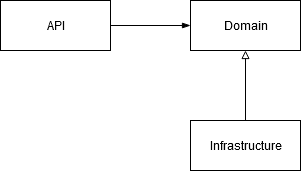
\includegraphics[width=0.5\textwidth]{images/domain-driven-design}
%\caption{Domain-Driven Design}
%\end{figure}

Im Laufe der Entwicklung stellte sich heraus, dass sich das Pattern, welches eigentlich für DotNet-Anwendungen konzipiert wurde, nicht so einfach auf die von uns verwendeten Programmiersprachen und Frameworks übertragen lässt.

Konkret, soll dies am Beispiel von Django, einem Python Web-Framework, verdeutlicht werden: Einer der Hauptzwecke der Infrastruktur-Komponente ist es die Anbindung verschiedener Datenbanken, sowie den Wechsel zwischen diesen so einfach und standardisiert wie möglich zu gestalten. In Django besteht dieses Problem allerdings garnicht, da die Datenbankanbindung komplett im Hintergrund stattfindet. Bei Verwendung des Django-REST-Frameworks entfällt außerdem ein Großteil der Arbeit, die zur Erstellung einer REST-API nötig ist, da auch hier vieles im Hintergrund passiert. Des weiteren gibt Django eine relativ umfassende Dateistruktur vor, die sich nur schwer mit dem Domain-Driven Design vereinen lässt. Aus diesen Gründen haben wir uns bereits zu einem frühen Zeitpunkt der Entwicklung entschieden dieses Pattern nicht länger als Orientierung zu nehmen.


\section{Frontend} % Klaus
% Deployment target: Cloud CDN
% Comparison to other hosting methods (pro/con)
% Ionic/Angular Stack > ready for mobile
% Easy-to-use WebSocket adapter
% Google OAuth login flow
% First throw. todo: verify and rephrase


\subsection{Technologie}
\label{sec:frontend-tech}

Hinsichtlich dem Ziel unsere Plattform einer möglichst großen Masse an Benutzern zugänglich zu machen, wird das Frontend mit Ionic (Version 5) entwickelt. Obwohl augenscheinlich nur Browser Technologien zum Einsatz kommen (HTML, CSS, JavaScript), kann die mit Hilfe von Ionic entwickelte Single-Page-App anschließend auch in eine native iOS bzw. Android App konvertiert werden. Intern fußt Ionic auf dem von Google propagierten Angular Framework, welches das \enquote{Two-way Binding} Paradigma umsetzt. Es unterstützt auch die von uns bevorzugte Programmiersprache TypeScript, ein Superset von JavaScript, sowie SASS als erweiterte Stylesheet-Sprache.

% \subsubsection{Datenstruktur in Ionic}

% In Ionic gibt es verschiedene Komponenten, die im Zusammenspiel die Anwendung komplett machen

% \subsubsection*{Page}

% Jede Ansicht einer Seite ist eine eigene Page. Die Page enthält ein HTML Template für die Ansicht, eine SCSS Datei für das Styling sowie eine TypeScript Datei für die Logik. Das HTML Template hat Zugriff auf Variablen und Funktionen der TypeScript Datei, um mit der Logik zu interagieren. Weiterhin gibt es für Jede Page Routing und Moduleinstellungen, um die Seite unter einer bestimmten URL erreichbar zu machen.

% \subsubsection*{Component}

% Eine Component ist ein Template, welches in Seiten oder anderen Components eingebunden werden kann. Somit können sich oft wiederholende Strukturen vereinheitlichen und mittels HTML Tag einbinden lassen. Components lassen sich auch Parameter übergeben, sodass diese Komponenten dynamisch verwendet werden können. Components bestehen ebenfalls aus HTML-Template, Styling und Logik. Ein Routing fehlt hier aber, sodass Components immer in Pages eingebunden werden müssen und nicht alleine stehen können.

% \subsubsection*{Service}

% Ein Service besteht nur aus dem Logikteil und kann von mehreren Pages eingebunden werden. So können Funktionen Global implementiert werden und Daten zentral verarbeitet werden.

% \subsubsection*{Pipes}

% Mit Pipes können Daten in einem HTML-Template transferiert werden, ohne eine Funktion aufrufen zu müssen. Ändern sich die zu transferierenden Daten, wird die Pipe automatisch neu angewendet.


\subsection{Authentifizierung}
\label{sec:frontend-auth}

\begin{figure}[H]
\centering
\label{fig:loginFlow}
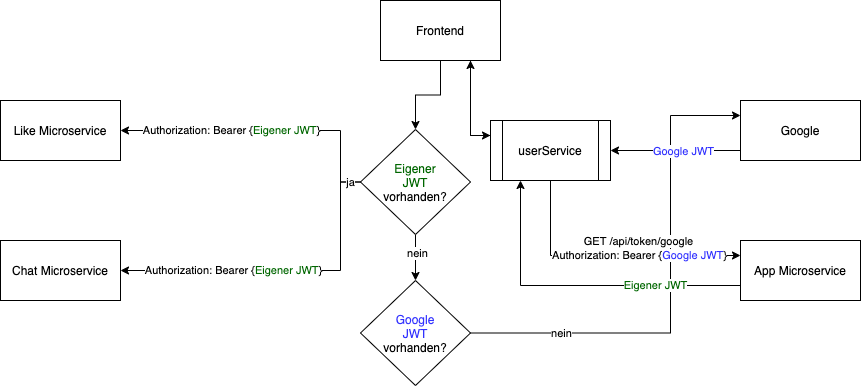
\includegraphics[width=\textwidth]{images/loginFlow}
\caption{Authentifizierung mit Google}
\end{figure}

% @TODO: authentication flow diagram
Die Authentifizierung eines Benutzers wird wie in Grafik \ref{fig:loginFlow} durchgeführt. Im ersten Schritt wird überprüft, ob bereits eine Session vorhanden ist. Diese ist durch das Vorhandensein eines gültigen JSON Web Token (JWT), ausgestellt vom
App-Microservice (siehe \autoref{sec:app-microservice}), gekennzeichnet. Andernfalls ist der Benutzer nicht eingeloggt. In diesem Fall, kann der Nutzer sich mit einem Social Provider (Facebook, Google, GitHub etc.) einloggen. Aktuell wird nur Google unterstützt. In jedem Fall wird jedoch eine OAuth 2.0 Anfrage an den jeweiligen Provider abgesetzt, die das Öffnen dessen Single Sign-On Fenster zur Folge hat. Bei erfolgreichem Ausweisen der Identität (normalerweise durch Benutzername und Passwort, ggf. mit OTP) liefert dieses ein sogenanntes ID Token zurück, das auch dem JWT Standard folgt. In dessen Payload findet sich neben den verifizierten Benutzer Details, wie Name oder Email Adresse, auch die in der Domäne des jeweiligen Provider eindeutige ID des Nutzers. Um den Login Vorgang abzuschließen, wird das ID Token an den App-Microservice gesendet, welches die Gültigkeit anhand der Signatur prüfen kann und dieses gegen ein neues JWT austauscht. Die Notwendigkeit für ein eigens ausgestelltes JWT wird in \autoref{sec:app-backend-auth} erläutert.

Genau genommen, handelt es sich bei der Antwort des App-Microservice um ein JWT-Paar, nämlich einem Access- und Refresh-Token. Das Access-Token wird für künftige Requests an jeden der Microservices als \texttt{Bearer} Token im \texttt{Authorization} Header mitgesendet, worauf basierend die Authentifizierung und Authorisierung in jedem Microservice stattfindet. Das Refresh-Token hingegen erlaubt es dem Frontend ein neues Access-Token zu erhalten, wenn dieses seine zeitliche Begrenzung überschritten hat. Refresh-Token sind in der Regel ein vielfaches länger gültig.

Um die Login-Session auch zwischen Neuladen der Webseite beizubehalten, werden beide Tokens im \texttt{localStorage} persistiert. Damit muss der oben beschriebene Login-Prozess erst wiederholt werden, wenn sich der Nutzer längere Zeit nicht im Portal bewegt hat und somit auch beide Tokens abgelaufen sind. Bei einem manuellen Logout werden beide Tokens zwangsläufig entfernt.


\subsection{Google OAuth Integration}

Zur einfachen Integration mit Angular, stellt Google das \texttt{gapi} NPM Package bereit. Es verwaltet den Zustand der Authentifizierung mittels eines \texttt{GoogleUser} Objektes, das auch eine Methode exponiert (\texttt{.getAuthResponse().id\_token}), um das in \autoref{sec:frontend-auth} erwähnte ID Token abzurufen. Sollte der Benutzer nicht angemeldet sein, kann der OAuth 2.0 Prozess durch die statische Methode \texttt{gapi.auth2.init()} gestartet werden. Diese Methode sollte mit der in der Google Developer Konsole konfigurierten \texttt{CLIENT\_ID} aufgerufen werden, um sicherzustellen, dass das ID Token aus dieser Login-Session und nicht der einer anderen Applikation stammt.


\subsection{Deployment}

Wie in \autoref{sec:frontend-tech} erläutert, besteht dieser Teil des Projekts lediglich aus einem Superset von Browser-Technologien (HTML, CSS, JavaScript). Es wird kein serverseitiger Code ausgeführt, somit ist auch kein Webserver erforderlich, um die Anwendung zu hosten. Stattdessen ist es ausreichend, das Frontend in einem öffentlichen read-only Dateisystem zu speichern. Hierfür eignet sich der Google Cloud Storage ideal. Um die Latenz noch weiter zu verringern, kann der Google Cloud CDN Service eingesetzt werden. Dies wiederum setzt einen HTTP(S) Load Balancer voraus, wie im Folgendem beschrieben.


\subsubsection{Google Cloud Storage}

Der Google Cloud Storage ist ein Cloud Speicher, um beliebige Binary Large Objects (BLOBs) zu speichern und in sogenannten Buckets (vgl. Ordner) zu verwalten. Es gibt kein Speicherlimit, stattdessen wird die Benutzung pro belegtem Gigabyte abgerechnet. Datensicherheit, Langlebigkeit sowie Verfügbarkeit werden durch die Google SLAs garantiert.

Mit dem Programm \texttt{gsutil} stellt Google eine Kommandozeilen-Schnittstelle zur Verfügung, über die auch der Frontend Bucket dieses Projektes regelmäßig aktualisiert wird.


\subsubsection{Cloud CDN \& Load Balancer}

Das Cloud Content Delivery Network (Cloud CDN) ist ein Netzwerk von Google, welches überall auf der Welt Knotenpunkte verteilt hat und damit auf die schnelle Auslieferung von Inhalten optimiert ist. Um dieses zu nutzen, muss ein HTTP(S) Load Balancer eingerichtet werden, der Anfragen an eine Domain erhält und diese an den jeweiligen Google Cloud Storage Bucket weiterleitet. Das Cloud CDN ist dazwischengeschaltet und fungiert als unabhängiger, automatischer Cache in mehreren Regionen der Welt.

Für die Skalierung bedeutet dieses Konstrukt, dass der Bucket nicht skalieren muss, denn Anfragen entstehen lediglich während dem CDN Cache-Refill bzw. beim Upload in den Bucket selbst. Bei einer steigender Anzahl von Nutzern muss nur das Cloud CDN skalieren. Hierfür sorgt Google vorbildlich.


\section{App-Microservice} % Arne
\label{sec:app-microservice}

Der App-Microservice stellt den Großteil der Backend-Funktionen unserer Anwendung bereit. Er ist in Python geschrieben, verwendet das Django Web-Framework und wird über Cloud Run bereitgestellt.


\subsection{Technologie}
\label{sec:app-tech}

Die Programmiersprache Python ergab sich aus der Wahl des Web-Frameworks. Django bietet einige entscheidende Bausteine, welche die Entwickelung von Web-Anwendungen vereinfachen und von denen auch wir großen Gebrauch gemacht haben.

Der vorzugsweise größte Vorteil ist die vollständige Abstraktion des Datenbankmodells durch das eingebaute Object-Relational Mapping (ORM). Dies ermöglicht das Anlegen und Verwalten einer SQL-Datenbank ohne echten SQL-Code schreiben zu müssen. Modelle und Relationen können mit Python-Code definiert werden, aus denen per Konsolen-Befehl sogenannte Migrations generiert, die anschließend von Django durch Umwandlung in SQL-Code auf die Datenbank übertragen werden. Entwickler können sich dadurch auf die reine Programmierung in Python konzentrieren.

Bei Zuhilfenahme des Django-REST-Frameworks werden auch die Standard REST-Funktionen (\texttt{GET}, \texttt{POST}, \texttt{DELETE}, etc.) für alle eigens angelegten Datenbank Modelle vor-implementiert, wodurch sich Entwickler umso mehr auf die für die Anwendung benötigten Funktionen konzentrieren können. Dieses Plugin erleichtert auch das Testen der Anwendung, in dem es eine Web Oberfläche zur Interaktion mit der API bereitstellt.

Daneben haben sich die eingebauten Konzepte, die Anwendung produktionsreif zu machen, schon mehrfach in der Industrie bewährt.


\subsection{Datenbank}
\label{sec:app-database}

Entsprechend dem Polyglott Persistency Prinzips, setzt der App Microservice auf eine Cloud SQL Instanz für relationale Daten, sowie einen Cloud Storage Bucket für Medien sonstiger Art (z.B. Fotos und Videos). Hinsichtlich dem SQL-Datenbank Typen, genügt MySQL (Version 8) unseren Anforderungen.

An dieser Stelle sollte erwähnt werden, dass zum Zeitpunkt der Entwicklung kein offizieller Emulator für den Google Cloud Storage vorliegt. Daher wurde zum Testen der Datenbankanbindung auf eine Open-Source Lösung namens \href{https://github.com/fsouza/fake-gcs-server}{\texttt{fake-gcs-server}} zurückgegriffen.


\subsection{Authentifizierung}
\label{sec:app-backend-auth}

Wie bereits in \autoref{sec:frontend-auth} dargelegt, knüpft die Nutzer-Authentifizierung an den OAuth 2.0 Flow eines jeweiligen Social Provider. Um den Login-Vorgang abzuschließen, muss das Frontend einen weiteren Request an den App-Microservice stellen, um das ID-Token des Social Provider gegen ein neues JWT zu tauschen, das von allen Services dieses Projektes akzeptiert wird. Dies hat zwei entscheidende Vorteile:

\begin{description}
	\item[Universally Unique Identifier (UUID)]
	\hfill \\
	Die im ID Token eines jeweiligen Social Provider gelistete Benutzer Identifikation (\enquote{\texttt{sub}} Payload-Claim) ist streng genommen nur in der Domäne des jeweiligen Social Provider eindeutig. Das heißt, ein Benutzer mit der Google ID \enquote{\texttt{xyz}} hat nicht zwangsläufig die gleiche ID bei Facebook und Co. Soll jedoch eine künftige Integration mit weiteren Single Sign-On Anbietern folgen, muss eine in der Domäne unserer Tiervermittlung eindeutige Benutzerkennung eingeführt werden.

	Zu diesem Zwecke, speichert der App-Microservice beim ersten Login mit dem ID Token eines jeweiligen Providers (z.B. \texttt{GET /api/token/google}) welche Kennung der Nutzer bei diesem Provider hat, legt zugleich aber auch für den Nutzer eine eindeutige UUID an, sodass ein Lookup in beide Richtungen künftig möglich ist.

	\item[Custom Claims]
	\hfill \\
	Ein Nebeneffekt von eigens ausgestellten JWTs ist die Tatsache, dass die Payload (\enquote{Claims}) der Tokens selbst festgelegt werden kann. Dies ist besonders für die Authorisierung anhand von \enquote{Scopes} relevant.
\end{description}

Damit dieses Token auch von den anderen Microservices zur Authentifizierung verwendet werden kann, exponiert der App-Microservice einen öffentlichen Endpunkt (\texttt{POST /api/token/verify}) mit dem die Gültigkeit eines solchen JWTs überprüft werden kann. In Produktion sollte diese Methode allerdings nicht verwendet werden, da sie unnötig zur Anfragenlast beiträgt. Stattdessen sollte lediglich der Public Key des Schlüsselpaars, mit dem die Signatur des JWTs erstellt wurde, öffentlich gemacht werden, sodass die anderen Services diesen initial laden und alle weiteren Schritte zum Prüfen der Gültigkeit lokal ausführen.


\subsection{Deployment}
\label{sec:app-deployment}

Schon bevor das Deployment Target (App Engine, Cloud Run, Kubernetes etc.) der einzelnen Microservices festgesetzt wurde, hat man sich darauf verständigt möglichst alle Dienste auf Container-Basis zu entwickeln. Das bedeutet, Code wurde prinzipiell immer gegen ein Linux-basiertes Container Image gebaut und getestet, mit dem garantiert werden kann, dass alle Entwickler die gleiche Entwicklungsumgebung vorliegen haben und Builds, sowie Fehler, leicht reproduzierbar sind, unabhängig von der zugrunde liegenden Hardware.

Es bietet sich daher an, auch ein Subset der Microservices als Container bereitzustellen. Dies ist auch der Fall für den App-Microservice.  Für das Container-basierte Deployment gibt es auf der Google Cloud Platform neben Kubernetes auch eine simplere Variante, nämlich Cloud Run. Beide sind in der Lage, basierend auf einer Deployment Spezifikation, die Container Anzahl entsprechend der Anfragelast zu skalieren.

Auch an dieser Stelle sei eine Limitierung der Google Cloud Plattform (vgl. \autoref{sec:app-database}) zu nennen. Eine Schwierigkeit, die uns beim Bereitstellen der Microservices, die Cloud Run benutzen, aufgefallen ist, stellt die fehlende Möglichkeit dar, eine SSH-Sitzung in einem laufenden Container zu starten. Somit kann eine Fehleranalyse nur schwer stattfinden. Log-basiertes Debugging kann nicht alle Problemquellen identifizieren. Uns ist weiterhin bekannt, dass andere Cloud-Anbieter diese Möglichkeit sehr wohl zur Verfügung stellen. Genau genommen bietet Google das mit seinem Kubernetes Dienst bereits indirekt an (\texttt{kubectl exec ...}). Zudem basiert Cloud Run auf Kubernetes. Dies kann sicherlich einen Einfluss auf die Wahl der Cloud-Plattform haben.


\section{Chat- und Like-Microservices} % Nik

Die Komponenten, die das Chatten zwischen Nutzern sowie das Liken von Angeboten ermöglichen, werden in diesen Abschnitt gemeinsam gelistet, da sie im Prinzip der gleichen Quelle entspringen, nämlich einem Monorepo.

Generell lässt sich sagen, dass beide dieser Services aus Gründen der Optimierung entstanden sind.

\subsection{Monorepo Strategie}

Mono-Repositories beschreiben eine Strategie bei der mehrere Projekte im gleichen versionierten Repository entwickelt werden. Dies bietet sich besonders bei Projekten an, die auf den gleichen Technologie-Stack setzen und hierdurch von einem vereinfachtem Dependency Management und leichterer Code Wiederverwendung profitieren können.

Ein solcher Ansatz erzwingt dennoch nicht das gleiche Deployment Target oder generell den gleichen Build Prozess. In diesem Falle wurden die Chat- und Like-Microservices als zwei Teilbereiche einer einzigen API konstruiert, die jedoch durch die selbst entworfene Plugin Architektur getrennt aktiviert und somit bereitgestellt werden können.

\subsection{Technologie}

Verglichen mit dem App-Microservice (siehe \autoref{sec:app-tech}), ist die Wahl der Programmiersprache nicht vom Framework geprägt, sondern von der Sprache selbst. Gerade hinsichtlich der Echtzeit-Kommunikation mit Browsern per WebSockets, ein Core-Feature des Chat-Microservices, hat sich JavaScript als Backend-Pendant über die Jahre bewährt.

Auf der anderen Seite, gibt es, vergleichen mit Django, im NodeJS Umfeld viel seltener Frameworks, die eine solch rigide Struktur ansetzen. Das wohl bekannteste, Express, ist absolut leichtgewichtig und eher als Routing Mechanismus mit Middleware zu verstehen. Für größere Projekte ist dies in unseren Augen aber auf lange zeit kontraproduktiv. Deshalb, haben wir glücklicherweise mit NestJS ein Framework gefunden, das den bewährten Konzepten von Angular folgt.

\subsection{Authentifizierung}

Die Authentifizierung setzt auf den in \autoref{sec:app-backend-auth} beschriebenen Mechanismus, um die vom App-Microservice ausgestellten JWTs zu verifizieren und danach die Identität des Nutzers zu ermitteln. Ein Spezialfall stellt die Authentifizierung des Echtzeit-Chats dar, wie in \autoref{sec:chat-microservice} ausgewiesen wird.



\subsection{Chat-Microservice}
\label{sec:chat-microservice}

% Deployment target: Cloud Run
% Storage: Firestore (emulator available)
% WebSocket authentication > not usable in upgrade request due to limited browser WebSocket API


\subsubsection{Datenbank}

Die Besonderheit des Chats liegt zum einen an der Anforderung diesen in Echtzeit anbieten zu können, zum Anderen, aber auch darin, dass sich das Format der Nachrichten populärer Messenger bekanntlich stark geändert hat. So ist es beispielsweise inzwischen möglich per WhatsApp sowohl reine Textnachrichten, als auch Links, Bilder oder Dokumente zu versenden. Keiner der Nachrichten-Typen lässt sich sinnvoll durch einen relationalen Datenbank Eintrag abbilden. Um auch unser Portal auf diesen Umstand vorzubereiten, setzen wir mit dem Chat-Microservice auf eine noSQL Datenbank, dem Google Firestore. Es handelt sich hierbei um eine Dokumenten-basierte Datenbank, die in Kollektionen aufgeteilt ist und im Grunde genommen JSON-Dokumente von max 1 MB speichert.


\subsubsection{Echtzeit-Chat}

\paragraph{WebSockets}

Effektiv unterliegt jeder dem für einen Browser bestimmten Nachrichtenverkehr dem HTTP Protokoll. Somit kommen auch nur eine Reihe von Technologien in Frage um Nachrichten in Echtzeit an Webseiten zu übertragen. Diese lauten:

\begin{itemize}
  \item HTTP (Long-)Polling
  \item HTTP Streaming
  \item Server-Sent Events
  \item WebSockets
\end{itemize}

Allerdings lassen sich nur mit WebSockets bidirektionaler Datenströme abbilden. Deshalb setzt dieser Teil der Anwendung auf diesen Transportkanal, der im NestJS Framework durch Gateways abstrahiert ist.


\paragraph{Skalierung}

Da WebSockets eine persistente Verbindung zwischen Client und Server einrichtigen, d.h. die Verbindung nicht wie traditionell nach jeder Anfrage schließen, sind besondere Vorkehrungen notwendig, um die Applikation horizontal zu skalieren. Denn es ist denkbar, dass ein Nutzer A, der mit Server-Instanz X verbunden ist, einem Nutzer B, der wiederum mit Server-Instanz Y in Verbindung steht, in Echtzeit eine Nachricht senden möchte. Dies bedarf der Kommunikation zwischen den horizontal skalierten Server-Instanzen X und Y. Hierfür setzt der Chat-Microservice auf Google Memorystore, einer In-Memory Datenbank, die zu 100\% dem Redis Protokoll folgt.

\paragraph{Authentifizierung}

WebSockets sind einzig und allein mit HTTP verwandet, in das dessen Handshake als eine Aufforderung zum WebSocket Upgrade verstanden werden kann. Das erlaubt es WebSockets mit traditioneller Web-Infrastruktur zu koexistieren. Theoretisch könnte über die Header der Upgrade Anfrage auch eine Authentifizierung implementiert werden, so wie in \autoref{sec:frontend-auth} beschrieben. Aus unerklärlichen Gründen bietet jedoch die Browser WebSocket Schnittstelle keine Möglichkeit Header zu definieren. Das funktioniert sehr wohl aus Sicht eines Backends. Deshalb implementiert dieser Teil der Anwendung eine Authentifizierung auf Applikationsebene. So kann sich im ersten Schritt jeder Client mit dem Chat WebSocket verbinden. Danach ist dieser aufgefordert eine \texttt{AUTH\_REQUEST} Nachricht mit seinem JWT zu verwenden. Das Token wird wie gewohnt geprüft. Erst dann wird der bereits geöffnete WebSocket zur Liste der authentifizierten Nutzer hinzugefügt und kann künftig Nachrichten erhalten.


\subsubsection{Deployment}

Das Deployment Target ist Cloud Run. Hinweise hierzu finden sich in \autoref{sec:app-deployment}.


\subsection{Like-Microservice}

% Deployment target: App Engine > comparison to Cloud Run
% Storage: BigTable (emulator available but not fully usable)

\enquote{Gefällt mir} Angaben haben über die Jahre wortwörtlich die Herzen der Nutzer erobert. Wir gehen deshalb davon aus, dass ein großer Teil der API Anfragen auf diese Domäne zurück zu führen sein wird. Im Umkehrschluss muss diese also individuell skalieren können.

Als Deployment Target ist aus rein experimentellen Gründen die Google App Engine vorgesehen. In Produktion würde auch dieser Microservice per Cloud Run bereitgestellt werden, so mal er bereits als Container Image vorliegt (vgl. \autoref{sec:app-deployment}).

Nennenswert ist zuletzt der gewählte Datenbank-Typ. Es handelt sich hierbei um Google Cloud BigTable, ein weiteres noSQL Produkt mit extrem niedriger Latenz und skalierbar bis auf Millionen Anfragen pro Sekunde. Im Kontext von \enquote{Gefällt mir} Angaben kann man sich die BigTable wie eine Excel Kalkulationstabelle vorstellen: für verschiedenen Angebote (Zeile) wird der \enquote{Gefällt mir} Zustand (Zelle) eines jeweiligen Nutzers (Spalte) nieder geschrieben. Dabei kann der Zustand der \enquote{Gefällt mir} Angabe durch einen Integer repräsentiert werden (\texttt{1 = Like} / \texttt{0 = Neutral} / \texttt{-1 = Dislike}). Die Angaben pro Angebot können durch die von Google bereitgestellten MapReduce Operationen effizient aggregiert werden.


\section{Recommender Cloud Function} % Savina
% Deployment target: Cloud Functions > benefits? when is it most cost efficient (high/low traffic)?
% Concept of using a dedicated DB view (vs. implementation of REST call [time-constraints])
% Trigger via PubSub > benefit to other trigger methods?
% Explain publishing via Google PubSub client form App Microservice
% Async nature of recommendation (not time critical or required to synchronous response when creating a new offer)
% Service token authentication (B2B communication)
% @TODO: why cloud function?

Gezeichnet von der Idee Benutzer über neue Angebote ihrer liebsten Rassen zu benachrichtigen, stellt die Cloud Recommender Function den einzigen Service dar, der nicht im Internet exponiert ist, d.h. keine frei zugängliche API hat. Stattdessen wird sie durch den Google Cloud PubSub Service ausgelöst. PubSub repräsentiert den asynchronen, ereignisgesteuerten Programmierstil bei dem Komponenten eines Systems Zustandsänderungen in Form von Events publizieren. Dabei ist im Allgemeinen nicht bekannt, welche anderen Komponenten diese Nachrichten empfangen werden oder wann sie diese verarbeiten. Letzteres stellt kein Problem dar, denn dieser Benachrichtigungs-Service wurde als nicht-zeitkritisches Feature definiert.

Auch gibt es unterschiedliche Ansätze dazu, wie aussagekräftig ein solches Ereignis ist. In diesem Anwendungsfall wäre es also denkbar, das komplette neu eingetroffene Angebot oder nur die ID dessen via PubSub zu publizieren. Weiterhin benötigt der Service Kenntnis darüber, welche Nutzer die Rasse des Angebots abonniert haben.

Aktuell geht die Recommender Cloud Function davon aus, dass das komplette Angebot publiziert wird. Verantwortlich dafür ist der App-Microservice (siehe \autoref{sec:app-microservice}). Intern, realisiert dieser das zuverlässige Publishing via PubSub durch einen \texttt{post-save} Hook auf die \enquote{Angebote} Tabelle der Datenbank. Basierend auf der im Angebot enthaltenen Rasse, kann die Recommender Cloud Function dann eine Liste der abonnierten Benutzer vom App-Microservice abrufen. In Produktion sollte diese doppelte Kopplung zum App-Microservice vermieden werden. Diese kann durch eine replizierte read-only Datenbank Instanz oder einer speziell angepassten Datenbank-View durchbrochen werden. In jedem Fall, kann die Cloud Function dann die abonnierten Nutzer per Chat-Microservice (siehe \autoref{sec:chat-microservice}) benachrichtigen. Durch das publizieren des gesamten neuen Angebots kann eine umfangreiche Nachricht (Name, Bilder, URL, etc.) an die Nutzer konstruiert werden.


\section{Security} % Savina
Bei der Implementierung wurde darauf geachtet, dass sowohl Betreiber als auch Nutzer gegen die gängigsten Angriffsvektoren geschützt sind. Das Abhören, Manipulieren oder Verletzen der Integrität von Daten darf nicht möglich sein. Im Folgenden werden entsprechende Lösungskonzepte präsentiert.


\subsection{Verschlüsselung der Kommunikation}
Eine unverschlüsselte Kommunikation zwischen Nutzer und Webserver bietet Angriffen wie dem Man-in-the-Middle Attack, Cross-Site-Scripting (XSS) und Session Hijacking ein breites Spielwfeld. Wir nutzen ausschließlich HTTPS, wodurch sämtliche Kommunikation verschlüsselt von statten geht und ein Angreifer keine Informationen extrahieren kann ohne die dem Zertifikat zugrunde liegende Public-Key Kryptographie zu brechen.


\subsection{Authentifizierung und Autorisierung}
\label{sec:authentication}

Die Nutzer Authentifizierung wurde ausführlich in \autoref{sec:frontend-auth} und \autoref{sec:app-backend-auth} ausgelegt. Sämtliche Kommunikation mit denen im Internet exponierten Services erfordert somit das Ausweisen der Identität, indem die von uns erstellen JWTs der jeweiligen Anfrage beigelegt werden müssen. Die Dauer der Gültigkeit der Access-Token ist frei konfigurierbar, standardmäßig jedoch auf 5 Minuten gesetzt. Auch die Authentifizierung unter den Services ist geregelt und erfordert spezielle Service Tokens. Jeder Microservice verwaltet hierzu eigenständig eine Whitelist und kann den Tokens darin eine Identität zuschreiben, wie z.B. der des Recommender Bot.

Auch die Authorisierung, also der Vorgang, ob ein gewisser Nutzer eine bestimmte Aktion ausführen darf, liegt im Verantwortungsbereich der Microservices. So darf beispielsweise kein Nutzer im Namen eines Anderen Nachrichten versenden oder Angebote hochladen.


\subsection{Weitere Lösungen}
Weitere Mechanismen zur Gewährleistung der Sicherheit sind:

\begin{itemize}
    \item Datenbankzugriffe erfolgen im App-Microservice ausschließlich über Django Queries. Diese sind vor SQL-Injektion geschützt, da ihre Abfragen mit Hilfe von Query-Parametrisierung konstruiert werden. Der SQL-Code einer Abfrage wird getrennt von den Parametern der Abfrage definiert. Da Parameter vom Benutzer bereitgestellt werden können und deshalb als unsicher gelten, werden sie vom zugrunde liegenden Datenbanktreiber escaped.~\cite{django-security}
    \item Im App-Microservice wurde eine Middleware eingerichtet, die Schutz gegen Cross-Site Request Forgery (CSRF) bietet.
    \item Da grundsätzlich kein User-Input in das Dateisystem einfügt wird, können Directory Traversal-Angriffe nicht stattfinden.
\end{itemize}

% Use table of attack vectors and detail how a protection mechanism was implemented

%\section{Scaling} % Klaus
% Load Balancer setup with serverless network endpoint groups > enables individual scaling
% Services and buckets may be deployed to multiple regions > LB decides which is the closets
% Some cloud resources must be in the same region in order to communicate > implications?
% Message broker for Chat microservice [Nik]
% Stateless REST enables horizontal scaling


\section{Continuous Integration und Delivery} % Arne + Nik

Beim Build und Deployment der verschiedenen Komponenten unserer Anwendung haben wir den Ansatz der Continuous Integration sowie der Continuous Delivery (CI/CD) verfolgt. Das bedeutet, neu eingecheckter Code wird kontinuierlich gegen existierenden geprüft, indem hierfür, sofern vorhanden, jedes Mal eine extensive Test Suite durchlaufen wird. Fehlerhafte Builds werden somit markiert und Pull Requests frühzeitig blockiert. Daneben lassen sich in diesem Integrations-Verfahren auch andere Schritte wie das Prüfen auf einen Styleguide oder Linter kombinieren. Basierend auf diesen ersten Qualitäts-Indikatoren, lässt sich eine Pipeline zur automatischen, kontinuierlichen Bereitstellung des neu eingecheckten Codes einrichten.

Mit GitHub Actions können beide dieser Konzepte umgesetzt werden. Denn neben der Git-basierten Versionierung von Code oder kollaborativen Tools wie Issues, Projects, Teams etc., bietet GitHub neuerdings einen kostenlosen Dienst an, um CI/CD an die Breite Masse seiner Open-Source Entwickler zu bringen. Die dafür notwendige Konfiguration wird samt Quellcode verwaltet. Allgemein tun wir das auch mit sonstigen Build Artefakten wie z.B. der Dockerfile oder Deployment Spezifikation eines jeden Microservices. Hierdurch gelingt uns ein vollumfängliches Bild zu jeder Version der Software, inklusive der Umgebung und Beschreibung wie diese Software gebaut und bereitgestellt wurde.


\section{Kostenanalyse}


\subsection{Annahmen zum Nutzerverhalten}

Verglichen mit anderen Plattformen, treffen wir die Annahme, dass es im Wesentlichen zwei Nutzergruppen gibt. Eine Gruppe nutzt die Anwendung vor allem zum Stöbern und Kaufen (\enquote{Interessenten}), die Andere nutzt sie zum Anbieten von Tieren (\enquote{Verkäufer}). Ein kleiner Anteil der Benutzer wird in beiden Rollen agieren. So kommen wir zu der Annahme, dass ein Benutzer im Durchschnitt zwei Inserate zu jedem Zeitpunkt online hat. Weiterhin gehen wir davon aus, dass jedes Angebot im Durchschnitt zwei Bilder und ein Video beinhaltet, was bei einer Größe von 2 MB pro Bild und 16 MB pro Video zu einem Gesamtspeicherplatz von etwa 20 MB pro Angebot führt.

Um den Datenverkehr zu berechnen, gehen wir davon aus, dass ein registrierter Benutzer pro Tag ein Angebot aufruft sowie fünf mal die Startseite besucht. Diese Zahl haben wie etwas höher angesetzt, da auch nicht registrierte Benutzer die Startseite aufrufen können und die Anzahl dieser Aufrufe schwierig vorherzusagen sind.

Tabelle \ref{tab:Parameters} fasst diese Annahmen zusammen.

\begin{center}\label{tab:Parameters}
\begin{tabular}{|l|l|}
    \hline
    Anzeigen pro Benutzer & 2 \\ \hline
    Speicherplatz pro Anzeige & 20 MB \\ \hline
    Datenverkehr pro Nutzer pro Monat & 600 MB \\ \hline
    Anzahl Likes pro Anzeige und Benutzer & 2 \\ \hline
    Anzahl Chats pro Benutzer pro Monat & 2 \\\hline
    Anzahl Nachrichten pro Chat & 6 \\\hline
    Größe einer Nachricht & 20 KB \\ \hline
\end{tabular}
\end{center}

\subsection{Auswertung}

Basierend auf den Werten in Tabelle \ref{tab:Parameters} kann man mit Hilfe des Google Cloud Platform Preisrechners einen ersten Kostenvoranschlag für die in unserem Projekt verwendeten Cloud Services erhalten~\cite{google-pricing}.

\FloatBarrier

\begin{figure}[H]
\centering
\label{fig:pricingUsers}
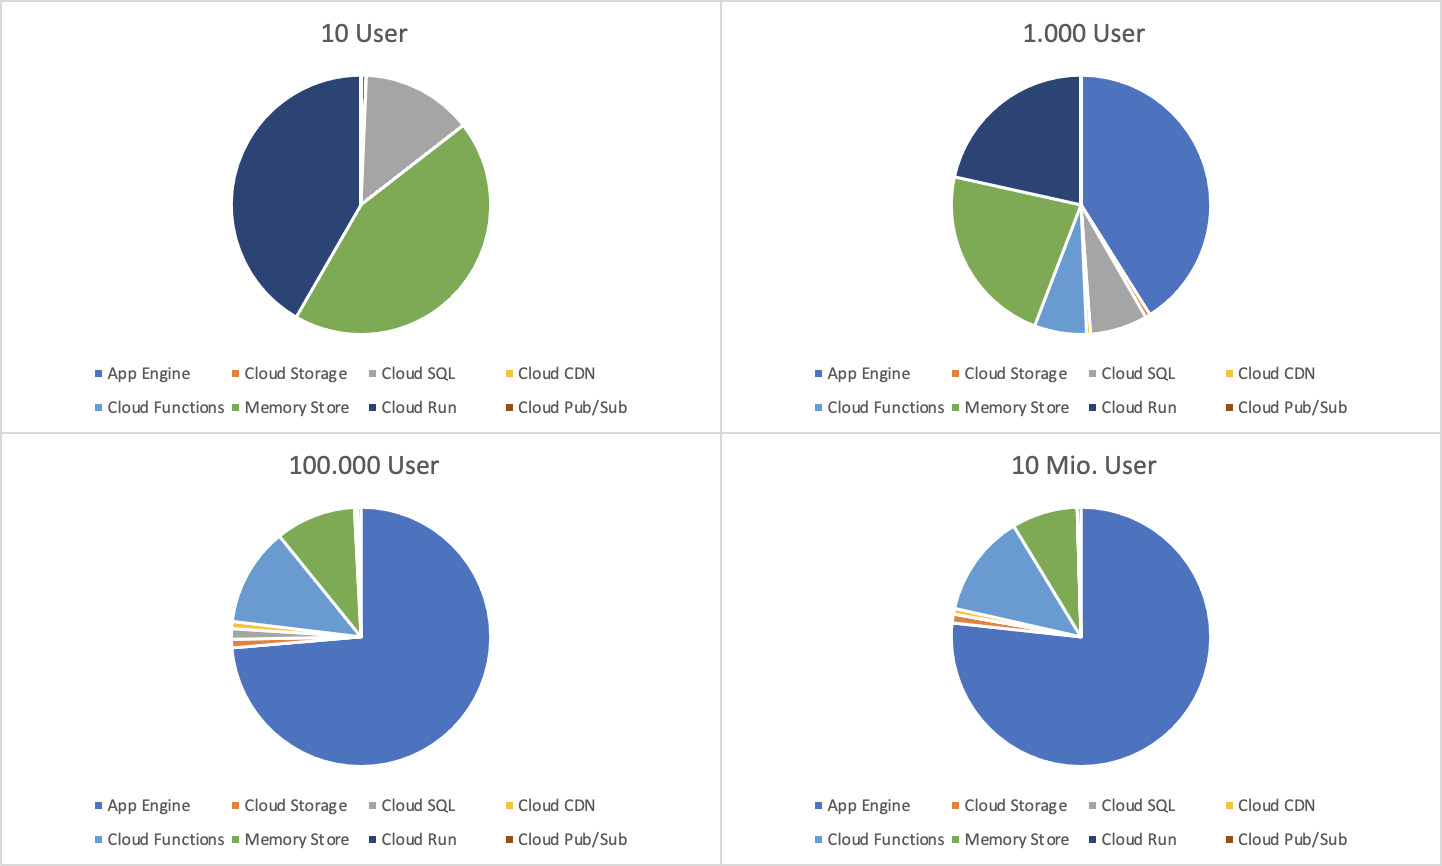
\includegraphics[width=\textwidth]{images/pricing-users}
\caption{Kostenanteil der einzelnen Services}
\end{figure}

Abbildung \ref{fig:pricingUsers} zeigt den Kostenanteil der Cloud Services im Verhältnis zu den Gesamtkosten. Hier ist besonders auffällig, dass mit steigender Zahl der Benutzer die Kosten für die App Engine einen größeren Anteil an den Gesamtkosten nehmen.

\FloatBarrier
\begin{center}\label{tab:totalCost}
    \begin{tabular}{|l||r|r|r|r|}
    \hline
         & 10 User & 1K User & 100K User & 10M User \\ \hline\hline
        Gesamtkosten & 73,10 \euro{} & 141,49 \euro{} & 7.906,20 \euro{} & 758.830,45 \euro{} \\ \hline
        Gesamtkosten pro User & 7,31 \euro{} & 0,14 \euro{} & 0,08 \euro{} & 0,08 \euro{} \\ \hline
    \end{tabular}
\end{center}

Um aussagekräftige Werte zu den Gesamtkosten zu erhalten, haben wir in Tabelle \ref{tab:totalCost} neben den Gesamtkosten zusätzlich die Kosten pro Benutzer in der jeweiligen Gruppe berechnet. Hier ist deutlich erkennbar, dass die Kosten pro Benutzer mit steigender Anzahl immer geringer werden. Das liegt vor allem daran, dass gewisse Cloud-Dienste unabhängig von der Anzahl der Benutzer, also als Fixpreis, berechnet werden. Mit steigender Zahl der Benutzer sinken somit die Fixkosten und damit auch die Gesamtkosten pro Benutzer.

\newpage

\appendix

% Swagger Docs (JSON export / links to production)
% Screenshots
% Larger architecture diagrams
% Individual service diagrams
% Google Cloud specific deployment diagram

\newpage

\bibliography{sources.bib}{}
\bibliographystyle{plain}

\end{document}
